\newcommand{\stern}{{\color{red!90!black}$\bigstar$}}
\newcommand{\raute}{{\color{blue}$\blacklozenge$}}
\newcommand{\pfeil}{\mbox{\color{blue}$<\hspace*{-.5em}\raisebox{0mm}{$\times$}\hspace*{-1em}\sqsupset$}} 

\documentclass[output=paper]{LSP/langsci}
\author{Tatiana Serbina, Paula Niemietz, Stella Neumann}
\title{Development of a keystroke logged translation corpus}
%\epigram{Change epigram in chapters/01.tex or remove it there }
\abstract{This paper describes the development of a keystroke logged translation corpus containing both translation product and -process data. The initial data comes from a translation experiment and contains original texts and translations, plus the intermediate versions of the unfolding translation process. The aim is to annotate both process and product data to be able to query for various features and recurring patterns. However, the data must first be pre-processed to represent individual keystroke logging events as linguistic structures and align source, target and process units. All process data, even material that does not appear in the final translation product, is preserved, under the assumption that all intermediate steps are meaningful to our understanding of the translation process. Several examples of possible data queries are discussed to show how linguistically informed quantitative analyses of the translation process data can be performed.}
\maketitle

\begin{document}
 
\section{Introduction}
Empirical translation studies can be subdivided into the two main branches, namely product- and process-based investigations \citep[see][]{Laviosa2002,Göpferich2008}. Traditionally, the former are associated with corpus studies, while the latter require translation experiments. The present study combines these two perspectives on translation by treating the translation process data as a corpus and tracing how linguistic phenomena found in the final product have developed during the translation process.
Typically product-based studies consider translations as texts in their own right, which can be analyzed in terms of translation properties, i.e. ways in which translated texts systematically differ from the originals. The main translation properties analyzed so far include simplification, explicitation, normalization towards the target text (TT), levelling out \citep{Baker1996} and shining through of the source text (ST) \citep{Teich2003}. Investigations into these properties can be conducted using monolingual comparable corpora containing originals and translations within the same language \citep[e.g.][]{Laviosa2002}, bilingual parallel corpora consisting of originals and their aligned translations \citep{Becher2010}, or also a combination of both \citep{Culo2012,Hansen-Schirra2012}.

Empirical research requires not only description but also explanation of translation phenomena. Why, for instance, are translated texts more explicit than originals? It has been suggested that explicitation as a feature of translated texts is a rather heterogeneous phenomenon and can be subdivided into four different types: the first three classes are linked to contrastive and cultural differences, whereas instances of the fourth type are specific to the translation process \citep[82-83]{Klaudy1998}. Other researchers propose to explain translation phenomena in general through contrastive differences between ST and TT, register characteristics and a set of factors connected to the translation process, for instance those related to the process of understanding \citep{Steiner2001}. Thus, studies using parallel corpora have shown that the majority of examples of explicitation found in the data can be accounted for through contrastive, register and/or cultural differences \citep{Hansen-Schirra2007,Becher2010}. Based on these corpus-based studies researchers can formulate hypotheses that ascribe the remaining instances to the characteristics of the translation process, and then test these hypotheses by considering data gathered during translation experiments, e.g. through keystroke logging. Keystroke logging software such as Translog \citep{Jakobsen1999} allows researchers to study intermediate steps of translations by recording all keystrokes and mouse clicks during the process of translation. Based on this behavioral data and the intermediate versions of translations, assumptions with regard to cognitive processing during translation can be made. Analysis of translation process data helps explain the properties of translation products, describe potential translation problems and identify translation strategies.

Previous studies in this area have focused on analysis of pauses and the number as well as length of the segments in between \citep[e.g.][]{Dragsted2005,Jakobsen2005,Alves2009,Alves2011}. Furthermore, translation styles have been investigated in both quantitative and qualitative manners \citep[e.g.][]{Pagano2008, CarlandDragsted2011} for example, the performances of professional and student translators have been compared with regard to speed of text production during translation, length of produced chunks and revision patterns \citep[e.g.][]{Jakobsen2005}.
 
In order to generalize beyond individual translation sessions and individual experiments, keystroke logging data has to be treated as a corpus \citep{Alves2004, Alves2009, Alves2011}. In other words, the data has to be organized in such a way as to allow querying for specific recurring patterns \citep{Carl2009} which can be analyzed both in terms of extra-linguistic factors such as age and gender of the translator or time pressure, as well as linguistic features such as level of grammatical complexity or word order. The latter research questions require additional linguistic annotation of the keystroke logging data (see Section 1.3). Thus, the aim of the present study is to create a keystroke logged corpus (KLC) and to perform linguistically informed quantitative analyses of the translation process data.

Section 2 describes the translation experiment data which serves as a prototype of a keystroke logged corpus, as well as the required pre-processing and linguistic annotation necessary for corpus queries, which are introduced in Section 3. A summary and a short outlook are provided in Section 4\footnote{This project is funded by the Excellence Initiative for the German State and Federal Governments.}. 

\section{Keystroke logged corpus}
\subsection{Data}

The first prototype of the keystroke logged translation corpus is based on the translation process data collected in the framework of the project PROBRAL\footnote{The project was funded by CAPES-DAAD PROBRAL (292/2008).} in cooperation with the University of Saarland, Germany and the Federal University of Minas Gerais, Brazil. In the translation experiment participants were asked to translate a text from English into German (into their L1).No time restrictions were imposed. The data from 16 participants is available: eight of them are professional translators with at least two years of experience and the other eight participants are PhD students of physics. Since the source text is an abridged version of an authentic text dealing with physics (see Appendix), the second group of participants are considered domain specialists. The original text was published in the popular-scientific magazine \textit{Scientific AmericanOnline}, and the translation brief involved instructions to write a translation for another popular-scientific publication. The text was locally manipulated by integrating ten stimuli representing two different degrees of grammatical complexity, illustrated in (1) and (2). Based on the previous research in the Systemic Functional Linguistics \citep[see][715]{Halliday2014}, \citep[8-10]{Taverniers2003} we assume that in the complex version the information is more dense and less explicit. For instance, whereas the underlined stretches of text in (1) and (2) contain the same semantic content, its realization as a grammatical clause in (1) leads to an explicit mention of the agents, namely the researchers, which are left out in the nominalized version presented in (2). During the experiment every participant translated one of the two versions of the text, in which simple and complex stimuli had been counterbalanced. In other words five simple and five complex stimuli integrated into the first source text corresponded to the complex and simple variants of the same stimuli in the second text. The only translation resource allowed during the translation task was the online bilingual dictionary leo\footnote{\url{http://dict.leo.org/ende/index_de.html} (accessed: 09.2014)}. The participants’ keystrokes, mouse movements and pauses in between were recorded using the software \textit{Translog}. Additionally, the information on gaze points and pupil diameter was collected with the help of the remote eye-tracker Tobii 2150, using the corresponding software \textit{Tobii Studio}, Version 1.5 \citep{Tobii2008}. Currently the corpus considers only the keystroke logging data, but later the various data sources will be triangulated \citep[see][]{Alves2003} to complement each other. The discussion of individual queries and specific examples in Section 3 indicates how the analysis of the data could benefit from the additional data stream. 

%\begin{figure}
%\includegraphics[width=1\textwidth]{./figures/2-0.png}
%\end{figure}

\begin{enumerate}[(1)]
\item Simple stimulus \newline
Instead of collapsing to a final fixed size, the height of the crushed ball continued to decrease, even three weeks \textit{after the researchers had applied the weight}. (Probral Source text 2)
\item Complex stimulus \newline
Instead of collapsing to a final fixed size, the height of the crushed ball continued to decrease, even three weeks \textit{after the application of weight}. (Probral Source text 1)
\end{enumerate}

The prototype of the KLC thus consists of 2 versions of the original (source texts), 16 translations (target texts) as well as 16 log files (process texts). The source and target texts together amount to approximately 3,650 words, not including the process texts. The total size taking into account various versions of the same target text words can be determined only after completion of the pre-processing step (see Section 2.2). All the texts belong to the register of popular scientific writing. After the gold standard is established, the corpus will be extended to include data from further translation experiments, e.g. those stored in the CRITT TPR-Database \citep{Carl2012}. The database is a collection of keystroke logging and eye-tracking data recorded during translation, editing and post-editing experiments. It provides both raw and processed data: for instance, originals and final translation products are tokenized, aligned and annotated with parts of speech, whereas the process data is analyzed in terms of gaze and keystroke units \citep{Carl2012}. According to the website, the current version of the database consists of approximately 1300 experiments\footnote{\url{bridge.cbs.dk/platform/?q=node/18} (accessed: 09.2014).}. In the development of our keystroke logged translation corpus wego further by identifying all potential tokens produced during a translation process and enriching these with linguistic information. At the moment, the relatively small size of the corpus is sufficient to develop the new procedures and queries required for this type of data. 

\subsection{Pre-processing}
While originals and the final translations can be automatically annotated and aligned using existing tools, the process texts require pre-processing before they can be enriched with further information. The keystroke logs consist of individual events corresponding to one press of a key or a mouse. To link this behavioral information to the linguistic level of analysis, the events have to be represented in terms of complete tokens. Since the intentions of a translator are not always clear, it is essential to reflect all possible tokens produced during the translation process. Using a modified version of the concept of target hypotheses that \citet{Lüdeling2008} introduced for learner corpora (which also contain non-standard language with errors), the KLC will include multiple layers of annotation reflecting different versions of the same tokens that could be inferred from the process data. Thus, in our context target hypotheses represent potential translation plans. Several hypotheses are annotated when the keystroke logging data is ambiguous, i.e. in cases when, based on the pressed keys, it is unclear what token the translator intended to produce and when the process contains additional indicators of increased cognitive processing such as longer pauses or corrections. This method retains the necessary level of objectivity because it does not force the researcher to select only a single version which appears most plausible at a certain stage of corpus compilation.

\citet{Leijten2012} discuss the processing of monolingual keystroke logging data by aggregating it from the character (keystroke) to the word level \citep[see also][]{Macken2012}. For translation data, however, the required processing is more complex: within the target text keystrokes are aligned to tokens, and these tokens (representing intermediate versions of words either preserved in the TT, or modified/deleted in the process) are in turn aligned to the alignment units consisting of ST-TT counterparts \citep[see][227]{Carl2009a}. The same process of alignment is also performed for the phrase and grammatical function levels. These alignment links make it possible to query for all intermediate versions of individual tokens and phrases (see Section 3.5).

To facilitate this alignment, an alignment tool was developed\footnote{The tool was developed by students Adjan Hansen (RWTH Aachen) and Chuan Yao (Georgia Institute of Technology) during aUROP project at RWTH Aachen University in 2013.}, which allows the researcher to manually select items to be aligned from the ST and the TT. These alignment units are saved in the same keystroke logging file. The screenshot in Figure 1 shows the selection of an alignment pair with the tool: the words \textit{explaining }from the ST list and \textit{erklären} ‘to explain’ from the TT list are highlighted to become alignment pair 0 in the bottom window. The window on the left part of the screen displays the XML file for reference.

\begin{figure}
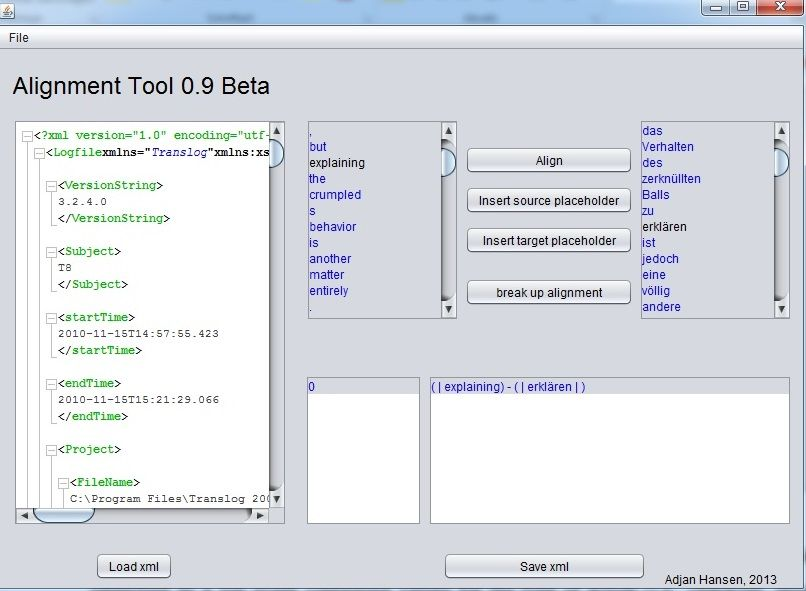
\includegraphics[width=.8\textwidth]{./figures/2-1.jpg}
\caption{Screenshot of an alignment process using the alignment tool}
\end{figure}


The \textit{Translog} software supplies the keystroke data in XML format. Each keystroke is identified as a log event containing values for the type of action (i.e., character, deletion, movement, mouse click), the cursor position of this keystroke, a time stamp and a block ID which identifies the number of characters highlighted in the log event (e.g. when a segment is highlighted prior to being moved or deleted). During the pre-processing stage for the prototype, the XML data was enriched by aggregating the log events into plausible tokens to which a token ID was assigned. For each alignment level (currently only word level; in the future also phrase and grammatical function levels) a reference link was specified to link the object to the corresponding alignment unit created by the aligner. If the token did not appear in the final version and could not be linked to any existing alignment units, the reference link was designated as an empty link. In example (3) below the three words \textit{für Verwirrung sorgt} ‘causes confusion', which appear in an intermediate version of this sentence, are characterized by empty links: since the same semantic information is expressed in the final version through a different grammatical structure using non-related lexical items, namely \textit{nicht vollständig erklären können} ‘could not explain entirely', the tokens cannot be connected to any alignment units. The reference to the empty links ensures that the information contained in the intermediate versions is preserved in the data and can be queried. These tokens can only be linked on the level of units larger than words. The frequent use of semantically equivalent structures rather than structurally similar units requires alignment on multiple levels, as certain relations cannot be captured at the level of individual words.\footnote{The intermediate versions of German translations use special characters introduced in interlinear representation, which is one of the visualizations provided by the keystroke logging software Translog.  {\raute} - a space character, {\stern} -  approx.1 sec. pause, [{\stern}36.721]- a pause of 36 seconds, 721 milliseconds,{\pfeil} - a backspace character. The part of the original corresponding to the translation is written in italics. One or more intermediate versions (GT\textit{i}) and the final version (GT\textit{f}) of translations, if relevant for the discussion, are presented in their chronological order.}

\begin{figure}
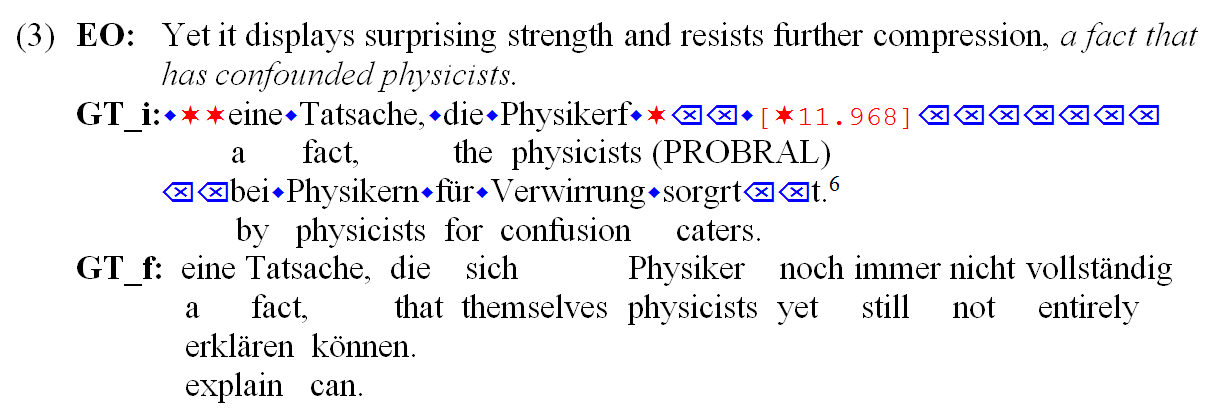
\includegraphics[width=1\textwidth]{./figures/2-3.png}
\end{figure}


%\begin{table}[h]
%\begin{tabular}{ll}
%\textbf{EO:} & Yet it displays surprising strength and resists further compression, \textit{a fact that} \\
% & \textit{has confounded physicists.} \\
% & {\raute}{\stern}{\stern}eine{\raute}Tatsache,{\raute}die{\raute}%Physiker{\raute}{\stern}{\pfeil}{\pfeil}{\raute}[11.968]{\pfeil}{\pfeil}{\pfeil}{\pfeil}{\pfeil}{\pfeil}{\pfeil} \\
% & a fact, the  physicists (PROBRAL)\\
% & {\pfeil}{\pfeil}bei{\raute}Physikern{\raute}für{\raute}Verwirrung{\raute}sorg{\pfeil}{\pfeil}t.\footnote{The intermediate versions of German translations use special characters introduced in interlinear representation, which is one of the visualizations provided by the keystroke logging software Translog.  {\raute} - a space character, {\stern} -  approx.1 sec. pause, [{\stern}36.721]- a pause of 36 seconds, 721 milliseconds,{\pfeil} - a backspace character. The part of the original corresponding to the translation is written in italics. One or more intermediate versions (GT\textit{i}) and the final version (GT\textit{f}) of translations, if relevant for the discussion, are presented in their chronological order.} \\
% & by physicists for confusion caters.\\
%GT\textit{f}: & eine Tatsache, die sich Physiker noch immer nicht vollständig \\
%              & a    fact, that themselves physicists yet still not entirely \\
% & erklären können \\
% & explain can.
%\end{tabular}
%\end{table}

%(3)	\textbf{EO:} Yet it displays surprising strength and resists further compression, \textit{a fact that has confounded physicists.}
%GT\textit{i}:\newline
%{\raute}{\stern}{\stern}eine{\raute}Tatsache,{\raute}die{\raute}Physiker{\raute}{\stern}{\pfeil}{\pfeil}{\raute}[11.968]{\pfeil}{\pfeil}{\pfeil}{\pfeil}{\pfeil}{\pfeil}{\pfeil}\newline
%a	fact, the  physicists (PROBRAL) \newline
%{\pfeil}{\pfeil}bei{\raute}Physikern{\raute}für{\raute}Verwirrung{\raute}sorg{\pfeil}{\pfeil}t.\footnote{The intermediate versions of German translations use special characters introduced in interlinear representation, which is one of the visualizations provided by the keystroke logging software Translog.  {\raute} - a space character, {\stern} -  approx.1 sec. pause, [{\stern}36.721]- a pause of 36 seconds, 721 milliseconds,{\pfeil} - a backspace character. The part of the original corresponding to the translation is written in italics. One or more intermediate versions (GT\textit{i}) and the final version (GT\textit{f}) of translations, if relevant for the discussion, are presented in their chronological order.}
%\newline by physicists for confusion caters.

%\item GT\textit{f}:\newline
%eine Tatsache, die sich Physiker noch immer nicht vollständig\newline 
%a fact, that themselves physicists yet still not entirely \newline 
%erklären können\newline
%explain can.\newline
       

Similarly, empty links were also defined in the ST-TT alignment units, if no corresponding element could be identified for either the ST or the TT \citep{Culo2012}, so that this information can also be extracted from the corpus.    

\subsection{Annotation}
“Corpus annotation adds value to a corpus in that it considerably extends the range of research questions that a corpus can readily address” \citep[29]{McEnery2006} a systematic annotation of particular information types throughout a corpus enables researchers to search for and extract corpus examples based on certain criteria included in one or more annotation layers. At the moment all texts are annotated with meta-information specifying the participant ID, a version of the translated text and the group (translator/physicist). The meta-information will be extended to include further variables relevant for potential analyses of the translation process data, e.g. participant-specific metadata such as age or native language \citep[see][]{Hvelplund2012}. Furthermore, the KLC will contain several layers of linguistic annotation. The part of speech (POS) annotation of the process texts was done manually for some examples in the corpus prototype, but the aim is to perform this step automatically for process as well as source and target texts through the use of an existing tagger. Automatic syntactic parsing and annotation of grammatical functions\footnote{Different taggers and parsers will be tested, and in a later step trained to accommodate the non-standard features present in the KLC. The ongoing work on pre-processing and annotation of monolingual process data \citep{Leijten2012,Macken2012} is being taken into consideration.} is also planned; however, it is recognized that manual interaction to check the results will still be necessary. The multilayer annotation \citep[see][]{Hansen-Schirra2006} will be extended by integrating the target hypotheses asa separate annotation layer (see Section 3.2). In addition, behavioral information such as the length of individual pauses \citep[see][]{Alves2009,Alves2011} will be annotated to facilitate quantifying these types of features, as well as querying for a combination of behavioral and linguistic information.

\section{Possible queries}
Depending on research questions, different types of queries into the translation process data are required. The following sub-sections describe a selection of possible queries: taking into account the novelty of this corpus type for translation process research, this section aims at showing the potential applications of the planned annotation and alignment layers introduced above for the analysis of translations.

\subsection{Alternative versions and incomplete structures within individual intermediate versions}
One query type concerns alternative versions of an unfolding target text. During the process of translation evolving texts typically undergo multiple revisions (e.g. in the form of deletions, overwrites or additions) before the final product is completed. One way of looking at revisions is to consider all keystrokes related to the translation of one source text sentence, up to the point where the translator begins translating other sentences, as an intermediate version of the translation of this source text sentence. The next version is identified, when and if the translation of this sentence is resumed after text production and/or revision of other passages\footnote{The identification of intermediate versions differs from the annotation of different target hypotheses (see Section 3.2): for instance, in (4) one intermediate version corresponds to two target hypotheses.}. Often such intermediate versions could function on their own: their linguistic structures are complete and could be left unchanged throughout the translation session. However, for various reasons, subsequent revisions may lead to (a series of) changes in these structures, thus creating new versions of the same sentences.

A single intermediate version may include several alternatives for the same linguistic slot realized by the same part of speech. For example, in (4) two versions of the modal verb within a subordinate clause have been supplied by the translator: the first of these in the present (\textit{können} ‘can’) and the second in the past tense (\textit{konnten} ‘could’), separated by a slash.\newline 


\begin{figure}
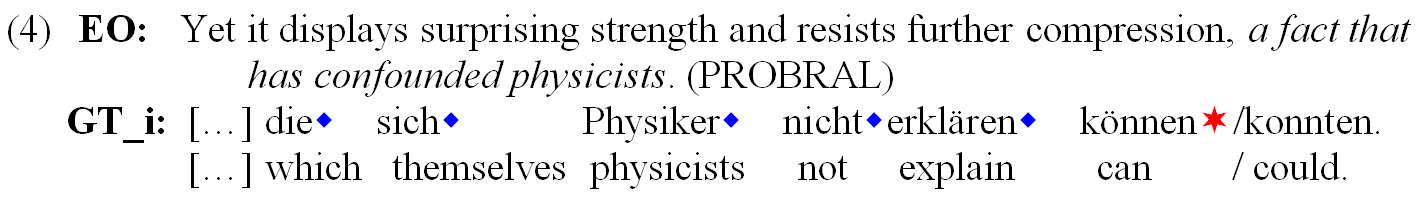
\includegraphics[width=1\textwidth]{./figures/2-4.png}
\end{figure}

%(4)
%\newline
%\textbf{EO:} Yet it displays surprising strength and resists further compression, \textit{a fact that has confounded physicists}.(PROBRAL)
%\newline
%GT\textit{i}:\newline
%[…] die{\raute}sich{\raute} Physiker{\raute}nicht{\raute}erklären{\raute}können{\stern}/konnten.\newline
%[…] which themselves physicists not explain can / could.
%\newline  

The part of speech annotation allows us to query this and similar patterns through a search for identical parts of speech separated by a punctuation mark. 
Figure 2 shows the XML code provided by the keystroke logging software Translog corresponding to the production of the tokens \textit{können} and \textit{konnten} in example (4). As can be seen, the tool generates files representing one log event (e.g. a keystroke corresponding to a letter or a slash) per line. The pre-processing step requires the grouping of these events into tokens, such as \textit{können} and \textit{konnten} in this example, which can be then annotated with part of speech tags. Here we use the tags from the Stuttgart-Tübingen Tagset (STTS) for German \citep{Schiller1999} for the purposes of illustration. Both \textit{können} ‘can' in Token 38 and \textit{konnten} ‘could' in Token 40 bear the part of speech tag VMFIN indicating “verb finite, modal”. 

\begin{figure}
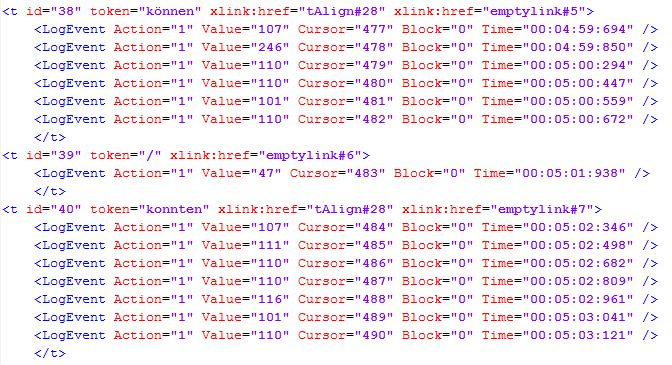
\includegraphics[width=.8\textwidth]{./figures/2-2.jpg}
\caption{XML code enriched with alignment links and information on tokens and parts of speech}
\end{figure}


Sometimes, alternatives might fill not only one part of speech slot but a whole phrase or clause, requiring a different approach in order to query for such more complex intermediate versions. The present study differentiates between words occurring in the ST and the TT, on the one hand, and different tokens that can be identified in the intermediate versions. From the perspective of the process all meaningful items in the intermediate versions are tokens. In addition, those tokens that are kept in the final translation are designated as words. This distinction helps us keep the process and the product of translation apart and study their interrelations: e.g. combinations between one or several words and a larger number of tokens, present in the same intermediate translation version, are considered to be an indicator that several alternatives for the same linguistic unit are included. Querying for such combinations would result in a more complete list of examples similar to (4).
 
However, in some cases a translator leaves a stretch of text unfinished by either writing more or less linguistic material than is required for a complete linguistic structure. Rather than adding multiple alternatives to a single translation version, a translator may also write an incomplete structure, in which a placeholder is substituted for the later linguistic unit, such as a sequence of characters ‘xxx’ or simply several space characters, as is shown in (5). In this sequence of word classes ART ADJA * KON VVFIN (article adjective * coordinating conjunction finite verb), the head noun of the noun phrase is missing. For this reason, searches for such examples also require POS annotation of the intermediate versions.

\begin{figure}
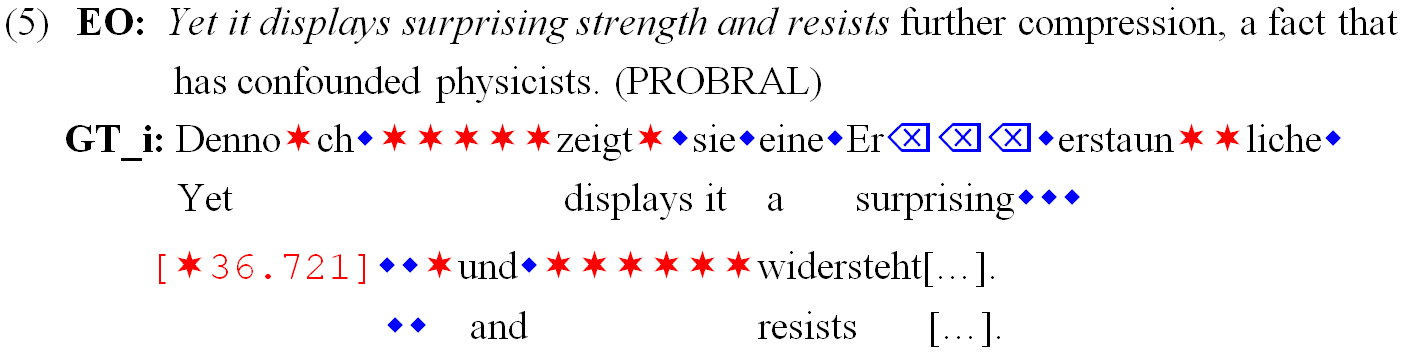
\includegraphics[width=1\textwidth]{./figures/2-5.png}
\end{figure}

%(5) \textbf{EO:} \textit{Yet it displays surprising strength and resists} further compression, a fact that has confounded physicists. (PROBRAL)
%\begin{itemize}
%\item GT\textit{i}:\newline
%Denno{\stern}ch{\raute}{\stern}{\stern}{\stern}{\stern}{\stern}zeigt{\stern}{\raute}sie{\raute}eine{\raute}Er{\pfeil}{\pfeil}{\pfeil}erstaun{\stern}{\stern}liche{\raute}\newline
%Yet displays it a surprising{\raute}{\raute}{\raute}\newline
%[{\stern}36.721]{\raute}{\raute}{\stern}und{\raute}{\stern}{\stern}{\stern}{\stern}{\stern}{\stern}widersteht[…].\newline
%{\raute}{\raute}and resists […].
%\end{itemize}\newline

Examples of the phenomena described in this sub-section can be seen as indications of understanding difficulties or attempts at finding the most suitable translation of the ST unit: the translator is aware of the problems and, rather than taking the time to optimize this section at that point, s/he prefers to continue translating the text, intending to return to this passage later. These examples can be investigated in terms of the translation strategies that are employed by translators. It is possible that the strategies differ not simply from translator to translator, but also depending on linguistic factors such as the grammatical complexity of the original.

\subsection{Alternative target hypotheses}
As mentioned earlier, some tokens found in the intermediate versions may be ambiguous: in these cases, the researcher cannot determine the intention of the translator. Here it is essential not to interpret the data but rather reflect all possible options by annotating several target hypotheses \citep{Lüdeling2008}. In example (6) the preposition \textit{innerhalb} and the indefinite article \textit{eines} is followed by a longer pause, after which the ending of the article is changed, turning \textit{eines} into \textit{einer}. Since articles in German contain morphological endings expressing the grammatical categories of person, number, gender and case, one different letter can affect the grammatical structure of the noun phrase. The researcher can, therefore, formulate a target hypothesis that the original plan for the noun phrase is \textit{eines Zylinders} ‘a{\tiny GEN.M} cylinder’, where the masculine genitive form of the determiner (matching the masculine noun) is typed, after which the translation plan changes. As a result, the translator deletes the –\textit{s} at the end of \textit{eines}, types the –\textit{r} instead (yielding the feminine form of the determiner \textit{einer}) and continues typing to produce the feminine noun \textit{Zylindergeometrie} ‘a{\tiny GEN.F} cylinder geometry’. Although only the token \textit{Zylindergeometrie} is evident at this point in the translation process, the existence of the assumed first version is supported by the fact that, at a later stage of the translation process, \textit{Zylindergeometrie} was altered to \textit{Zylinder}. It is plausible that the text-editing operations leading to a different grammatical suffix –especially if preceded by a longer pause (a potential indicator of increased cognitive processing \citep[see][]{Dragsted2005} – do not represent the correction of a simple typing error, but rather reflect a more complex cognitive process of changes to the translation plan. Still, the researcher cannot discount the possibility that the change from –\textit{s} to –\textit{r} is in fact a simple correction of a typo. This scenario constitutes another target hypothesis.

\begin{figure}
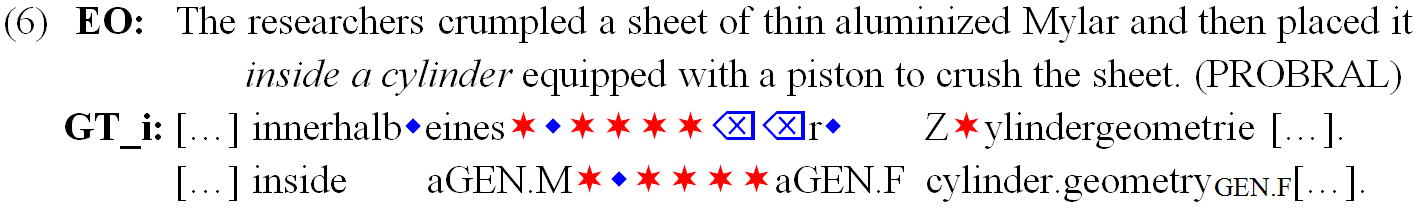
\includegraphics[width=1\textwidth]{./figures/2-6.png}
\end{figure}

%(6)	\textbf{EO:} The researchers crumpled a sheet of thin aluminized Mylar and then placed it \textit{inside a cylinder} equipped with a piston to crush the sheet.(PROBRAL)
%\begin{itemize}
%\item GT\textit{i}:\newline
%[…] innerhalb{\raute}eines{\stern}{\raute}{\stern}{\stern}{\stern}{\stern}{\pfeil}{\pfeil}r{\raute} Z{\stern}ylindergeometrie […].\newline
%[…] inside aGEN.M{\stern}{\raute}{\stern}{\stern}{\stern}{\stern}aGEN.F cylinder.geometryGEN.F[…].\newline
%\end{itemize}

Planned annotation of alternative target hypotheses\footnote{Since the notion of target hypotheses was originally developed for annotation of learner corpora, it has to be modified to be compatible with the translation process data.}  will allow querying for such patterns. These can be analyzed with regard to more or less technical vocabulary, as is the case in example (6), verbal or nominal variants, etc. Taking into account a number of explanatory factors, such as register characteristics or process-related variables, a comprehensive picture on such alternations will emerge. 

\subsection{Incorrect combinations of morphological markings in the final product}
Analyzing the final product in terms of its quality, the researcher may come across grammatical errors, as in (7). The grammatical rule in German requires that in noun phrases, not only articles and nouns but also premodifying adjectives agree in person, number, gender and case. For instance, in (7) the intermediate version contains the noun phrase \textit{eine dünne Alufolie} ‘a thin aluminium foil'. The head noun \textit{Alufolie} ‘aluminium foil' has the following characteristics: 3rd person singular, feminine gender and accusative case. Therefore, the indefinite article \textit{ein} ‘a' and the adjective \textit{dünn} ‘thin' are used with the ending -\textit{e} indicating the same person, number, gender and case. In the final version the corresponding NP has the form \textit{eine dünnes Blatt Alufolie} ‘a thin sheet of aluminium foil': here the head noun is no longer \textit{Alufolie} ‘aluminium foil' but rather the noun \textit{Blatt} ‘sheet', having the same person, number and case but different gender, namely neutrum. To agree with the head noun along these four paramaters, the ending of the adjective has been changed to -\textit{es} and the article should have been modified into \textit{ein} 'a-ACC.N'. However, this rule has not been observed.

\begin{figure}
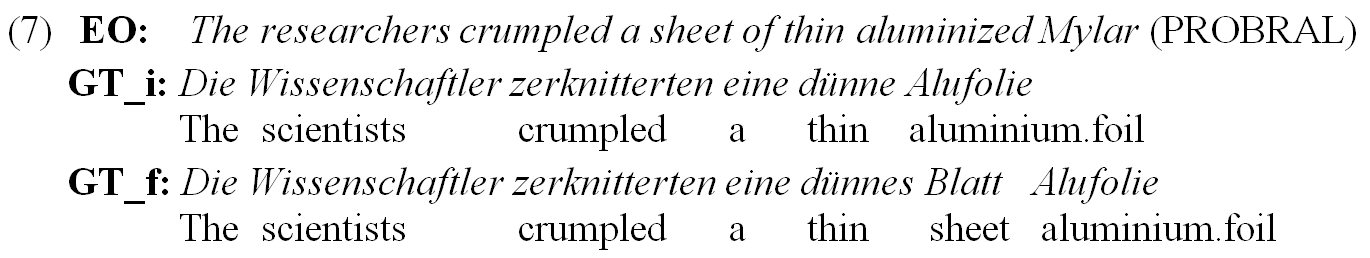
\includegraphics[width=1\textwidth]{./figures/2-7.png}
\end{figure}

%(7)	\textbf{EO:} \textit{The researchers crumpled a sheet of thin aluminized Mylar}(PROBRAL)
%\begin{itemize}
%\item GT\textit{i}: \textit{Die Wissenschaftler zerknitterten eine dünne Alufolie}\newline
%The  scientists crumpled a thin aluminium.foil
%\item GT\textit{f}: \textit{Die Wissenschaftler zerknitterten eine dünnes Blatt   Alufolie}\newline
%The  scientists crumpled a thin sheet aluminium.foil\newline
%\end{itemize}

Considering not only the source and the target text but also intermediate versions of translation helps understand how the grammatical error has been introduced into the final product: the noun phrase \textit{a sheet of thin aluminized Mylar} is initially translated to the noun \textit{Alufolie} ‘aluminium foil’ and then changed during a (later) revision phase into \textit{Blatt Alufolie} ‘sheet of aluminium foil’, which is more similar to the original than the first attempt: the level of explicitness of the ST is recreated by specifying that exactly one sheet of the foil rather than simply aluminium foil was crumpled. During this revision the morphological ending of the preceding adjective is changed to agree in gender with the new head noun \textit{Blatt} ‘sheet’, but the ending of the article is not modified accordingly. Since all translations were performed into the native language of test subjects, grammatical inconsistencies are not necessarily due to a lack of grammatical competence. One possible explanation could be that the increased cognitive effort during translation of this noun phrase leads to a grammatical error in the final version, possibly by drawing the cognitive resources away from the grammatical article. This hypothesis can be further tested by triangulating the keystroke logging data to such eye-tracking variables as number and length of fixations or pupil dilation, which are typically used in the eye-tracking research to operationalize cognitive demands \citep[e.g.][]{Pavlovic2009}.

\subsection{Substitutions of word classes}

Translation studies research has a long tradition of studying the phenomenon of translation shifts, i.e. various changes introduced during the translation process and visible in the translation product. A parallel corpus of aligned originals and translations allows a systematic analysis of shifts between translation units of various sizes and on different level of linguistic analysis. For instance, a recent corpus-based study has concentrated on shifts between different word classes \citep{Culo2008}, the so-called “transpositions” \citep[36]{Vinay1995/1958}. Example (8) illustrates a change from the verb require in the English original to the adjective \textit{erforderlich} ‘necessary’ in the final version of the German translation. 

\begin{figure}
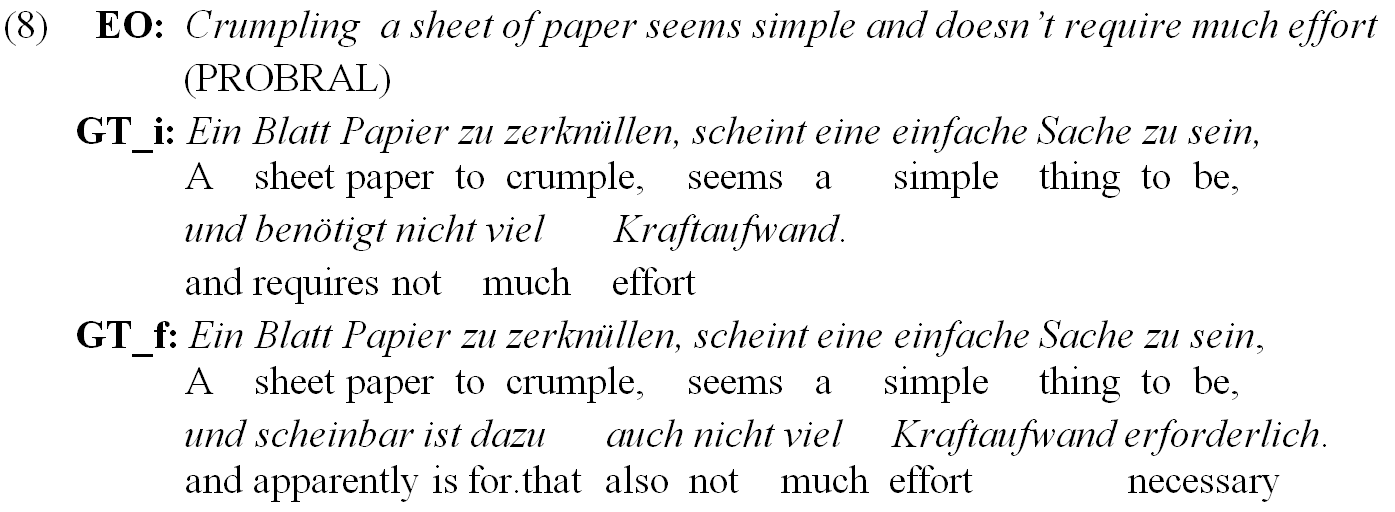
\includegraphics[width=1\textwidth]{./figures/2-8.png}
\end{figure}

%(8)	\textbf{EO:} \textit{Crumpling  a sheet of paper seems simple and doesn’t require much effort}(PROBRAL)
%\begin{itemize}
%\item GT\textit{i}:\newline
%\textit{Ein Blatt Papier zu zerknüllen, scheint eine einfache Sache zu sein,}\newline
%A sheet paper  to  crumple, seems a simple thing to be,\newline
%\textit{und benötigt nicht viel Kraftaufwand.}\newline
%and requires not much effort
%\item GT\textit{f}:\newline
%\textit{Ein Blatt Papier zu zerknüllen, scheint eine einfache Sache zu sein,}\newline
%A sheet paper to crumple, seems a simple thing to be,\newline
%\textit{und scheinbar ist dazu auch nicht viel Kraftaufwand erforderlich.}%\newline
%and apparently is for that  also  not    much  effort necessary \newline
%\end{itemize}

It is possible to extract this translation shift from a verb in the ST to an adjective in the TT using an available English-German parallel corpus such as CroCo \citep{Hansen-Schirra2012}. However, this kind of product-oriented corpus does not contain the information on what happens to the original verb in the intermediate translation versions. As is shown in (8), the translation shift was not introduced until a later revision of the pattern: the verb \textit{benötigen} ‘require’, initially used as a translation of the English verb, was replaced at a later stage by an adjective integrated into a different clause-level structure. The opposite pattern is also possible, in which a translation shift present in the intermediate version disappears during further editing of the translation. Thus, a keystroke logged corpus would enable researchers to extract shifts present at different stages of the translation development and to compare, for instance, the two possible revision patterns involving changes of word classes.
  
Previous studies have suggested that translation involves a process of understanding during which the semantic content of the ST has to be unpacked by the translator. In other words, it is assumed that certain highly dense grammatical structures are typically understood in terms of grammatically less complex patterns. A number of factors influencing translations, such as contrastive differences, register characteristics or other translation process-dependent variables (e.g. time pressure)might lead to changes with respect to the level of grammatical complexity of the corresponding TT unit, depending on how information is repacked by the translator \citep{Steiner2001,Hansen-Schirra2012}. Shifts of grammatical complexity have been operationalized as shifts of word classes. Thus, for example, the same semantic information can be expressed either as a clause or as a noun phrase; in the latter case the described event is presented in a more compressed manner, making certain aspects implicit. By looking at shifts between verbs and nouns, such changes of complexity can be analyzed further. The addition of intermediate versions allows the investigation of how often and under which circumstances the level of grammatical complexity is changed during the process of translation. 

\begin{figure}
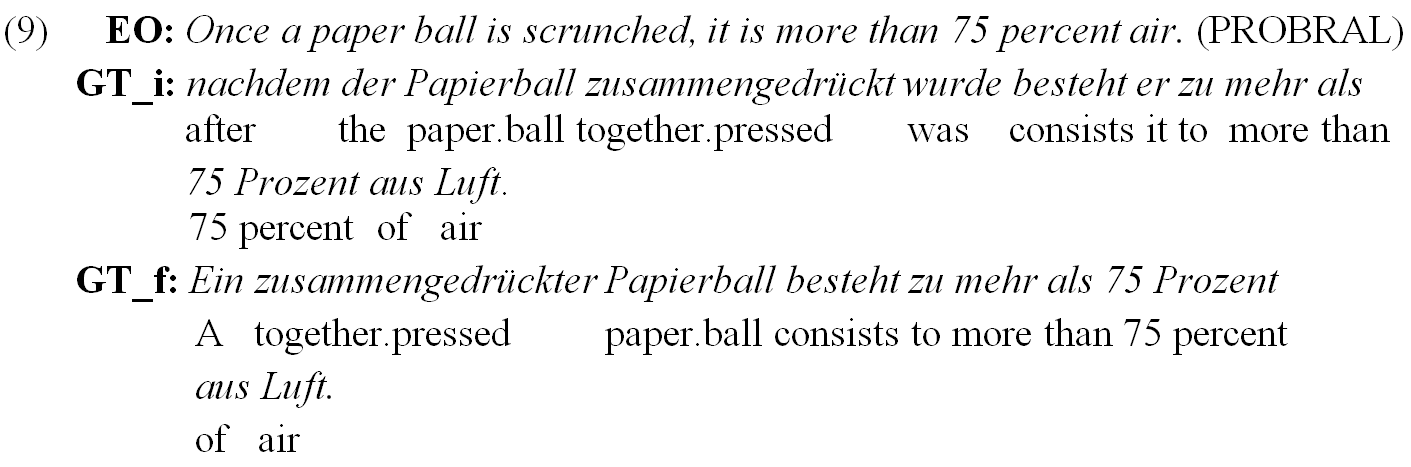
\includegraphics[width=1\textwidth]{./figures/2-9.png}
\end{figure}

%(9)	\textbf{EO:} \textit{Once a paper ball is scrunched, it is more than 75 percent air.} (PROBRAL)
%\begin{itemize}
%\item GT\textit{i}:\newline 
%\textit{Nachdem der Papierball zusammengedrückt wurde, besteht er zu mehr als}\newline
%after the  paper.balltogether.pressed was consists it to  more than\newline
%\textit{75 Prozent aus Luft.}
%75 percent  of   air

%\item GT\textit{f}:\newline 
%\textit{Ein zusammengedrückter Papierball besteht zu mehr als 75 Prozent}%\newline
%A   together.pressedpaper.ball consists to more than 75 percent\newline
%\textit{aus Luft.}\newline
%of air\newline
%\end{itemize}

In (9) a professional translator has initially kept the structure of the original sentence: a temporal adverbial expressed through a subordinate clause is present in both the ST and the intermediate version of the TT. However, during the final revision the clause is turned into an NP by using a strategy of premodification typical for German, namely a reduced participle clause. This compression of semantic information results in a more complex grammatical structure in the German translation than in the English original. It has been suggested that one of the factors leading to the increase of grammatical complexity could be high translation competence \citep[260]{Hansen-Schirra2012}. To test this hypothesis, the frequency of similar examples in translations by professional translators and physicists could be compared and submitted to statistical tests. 

\subsection{Lexical substitutions}
As mentioned in Section 2.2, the alignment units defined between corresponding words, phrases or chunks in the ST and the TT function as reference points to which the process tokens are linked during the pre-processing of the data. Using these reference links a researcher can trace the history of the TT word. While the previous section discusses an example in which a verb in the intermediate version is linked to an adjective in the final TT, a revision does not necessarily affect the grammatical structure of a sentence. Thus, as is shown in example (10), the changes could also be at a lower level of complexity: in this sentence only the noun slot is repeatedly modified before the translator finds a solution that s/he considers to be most suitable. This and similar instances found in the KLC are interpreted in terms of register characteristics or stylistic reasons (e.g. avoidance of repetitions).

\begin{figure}
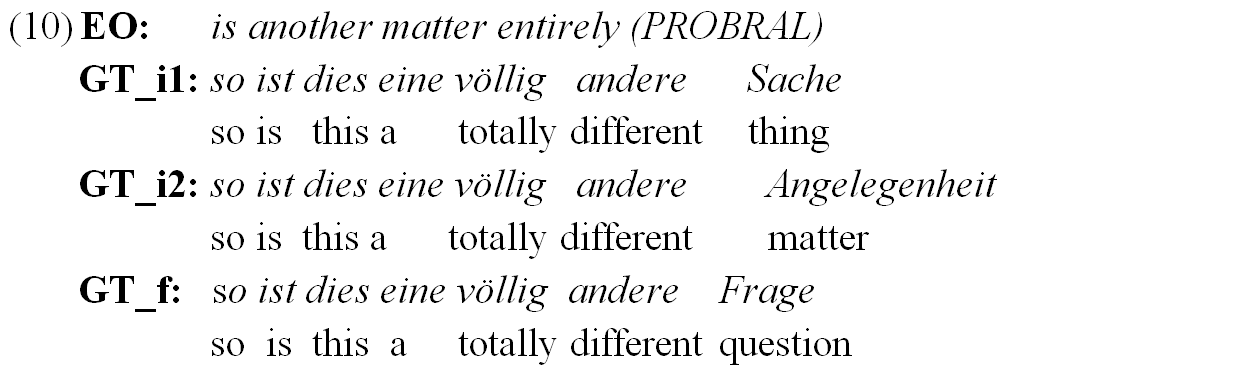
\includegraphics[width=1\textwidth]{./figures/2-10.png}
\end{figure}

%(10) \textbf{EO:} \textit{is another matter entirely} (PROBRAL)
%\begin{itemize}
%\item GT\textit{i}1:\newline 
%\textit{so ist dies eine völlig andere Sache}\newline
%so is this a totally different thing
%\item GT\textit{i}2:\newline
%\textit{so ist dies eine völlig andere Angelegenheit}\newline 
%so is  this a totally different matter
%\item GT\textit{f}:\newline
%\textit{so ist dies eine völlig andere Frage}\newline
%so is this a totally different question\newline
%\end{itemize}

This particular example illustrates that the alignment of process tokens involves a certain level of interpretation on the part of the researcher: according to \citet[92]{Kollberg2001}, “if a writer deletes a word, and subsequently inserts another word at the same position in the text, one cannot deduce that the writer intended the second word to replace the first (even if this is often the case)”. In other words, the authors indicate that though it might seem obvious to assume that the writer/translator meant to substitute a certain word, it is still an interpretation by the researcher and, therefore, does not belong to the formal level of data description; the functional analysis should be left to a later research stage \citep[92-93]{Kollberg2001}. The distinction between formal and functional data pre-processing can be compared to formal and functional types of annotation found in the corpora: for instance, on the formal level, sentences can be parsed into individual phrases, whereas an additional functional annotation would involve enrichment of these units with grammatical functions. The present study takes the position that both types of pre-processing and annotation are required. This combination of formal and functional levels facilitates different types of analyses. Thus, it is possible to analyze the data in a more qualitative manner by looking at individual sentences or texts: in this case the formal pre-processing of the keystroke logging data might be enough. At the same time, the queries discussed in this article are designed to conduct quantitative investigations, which certainly benefit from additional functional types of pre-processing and annotation. As long as all of the decisions involved in these processes are made transparent, the researcher can assess which information stored in the corpus is required for each individual case. 

\section{Conclusion and Outlook}
In this paper we have described the compilation and annotation of a keystroke logged corpus containing original and translated texts along with the process texts, with the aim of tracing the development of the linguistic phenomena found in the final product through the intermediate versions of the unfolding text during the translation process. This requires complex alignment procedures on several levels of analysis together with multilayer annotation to include information such as target hypotheses and typical translation features (e.g. grammatical shifts). The corpus will allow us to query the data to discover consistencies or compare intermediate versions to understand more about the translation process; thus, while it is particularly the quantitative research into the translation process that will be facilitated through this type of corpus, the interpretation of these quantitative findings requires taking a more qualitative perspective on the data.

The next steps in the development of the corpus are undertaken within the work of the RWTH Boost Fund project \textit{e-cosmos}. The goal of \textit{e-cosmos} is to develop a transparent and user-friendly environment for the quantitative analysis of complex, multimodal humanities data, and at the same time allow researchers to interact with the data, from the collection stage through (semi-automatic) annotation to the application of a wide range of statistical tests. This approach has two immediate consequences for the translation data: 1) the data outputs and formats generated by the parsers and other tools selected for work with the data will be compatible; and 2) the platform will enable the analysis of the keystroke data together with other data streams such as the eye-tracking data, thereby allowing more fine-grained quantitative analyses. The combined analysis of the data on translation process and product will contribute to a comprehensive understanding of the various factors playing a role in translation.  


\section{Appendix}

\subsection{Shortened original}
Crumpling a sheet of paper seems simple enough and certainly doesn't require much effort, but explaining why the resulting crinkled ball behaves the way it does is another matter entirely. Once scrunched, a paper ball is more than 75 percent air yet displays surprising strength and resists further compression, a fact that has confounded physicists. A report in the February 18 issue of Physical Review Letters, though, describes one aspect of the behavior of crumpled sheets: how their size changes in relation to the force they withstand.
 
A crushed thin sheet is essentially a mass of conical points connected by curved ridges, which store energy. When the sheet is further compressed, these ridges collapse and smaller ones form, increasing the amount of stored energy within the wad. Sidney Nagel and colleagues of the University of Chicago modeled how the force required to compress the ball relates to its size. After crumpling a sheet of thin aluminized Mylar, the researchers placed it inside a cylinder equipped with a piston to crush the crumpled sheet. Instead of collapsing to a final fixed size as expected, the team writes, the height of the crushed ball continued to decrease, even three weeks after the weight was applied […].
 
Scientific American Online, February 5, 2002, Sarah Graham: A New Report Explains the Physics of Crumpled Paper. \url{http://www.scientificamerican.com/article.cfm?id=a-new-report-explains-the}

\subsection{Source text 1}
Crumpling a sheet of paper seems simple and doesn't require much effort, but explaining \textit{why the crumpled ball behaves the way it does} is another matter entirely. \textit{A scrunched paper ball} is more than 75 percent air. Yet it displays surprising strength and \textit{resistance to further compression}, a fact that has confounded physicists. A report in Physical Review Letters, though, describes one aspect of the behavior of crumpled sheets: \textit{how their size changes} in relation to the force they withstand.
A crushed thin sheet is essentially a mass of conical points connected by \textit{curved energy-storing ridges. When the sheet is further compressed}, these ridges collapse and smaller ones form, increasing the amount of stored energy within the wad. Scientists at the University of Chicago modeled \textit{how the force required to compress the ball relates to its size. After the crumpling of a sheet of thin aluminized Mylar}, the researchers placed it inside a cylinder. They equipped the cylinder with a piston to crush the sheet. Instead of collapsing to a final fixed size, the height of the crushed ball continued to decrease, even three weeks after the application of weight.

\subsection{Source Text 2}
Crumpling a sheet of paper seems simple and doesn't require much effort, but explaining \textit{the crumpled ball’s behavior} is another matter entirely. Once a paper ball is scrunched, it is more than 75 percent air. Yet it displays surprising strength and \textit{resists further compression}, a fact that has confounded physicists. A report in Physical Review Letters, though, describes one aspect of the behavior of crumpled sheets: \textit{changes in their size} in relation to the force they withstand.

A crushed thin sheet is essentially a mass of conical points connected by \textit{curved ridges, which store energy. In the event of further compression of the sheet} these ridges collapse and smaller ones form, increasing the amount of stored energy within the wad. Scientists at the University of Chicago modeled \textit{the relation between compression force and ball size. The researchers crumpled a sheet of thin aluminized Mylar and then} placed it inside \textit{a cylinder equipped with a piston} to crush the sheet. Instead of collapsing to a final fixed size, the height of the crushed ball continued to decrease, even three weeks \textit{after the researchers had applied the weight}.

\printbibliography[heading=subbibliography,notkeyword=this]

\end{document}